\documentclass{article}
\usepackage[utf8]{inputenc}
\usepackage{xcolor}
\usepackage{booktabs}
\usepackage{multirow}
\usepackage{graphicx}
\usepackage{svg}
\usepackage{float}
\usepackage{biblatex} %Imports biblatex package
\usepackage[hidelinks]{hyperref}
\addbibresource{references.bib} %Import the bibliography file

\title{Neigh Corp - Golden Meadows}
\author{Marlen Baumgart \and Rodions Busurovs \and Carmen Silberbach \and  Martin Kashapov \and  Ludwig Temmel \and  Ilyas Yildirim}

\date{\today}

\renewcommand*\contentsname{Contents}

\newenvironment{boxed}
    {
    \begin{center}
    \begin{tabular}{|p{0.9\textwidth}|}
    \hline\\
    }
    { 
    \\\\\hline
    \end{tabular} 
    \end{center}
    }

\begin{document}
    \maketitle

    \tableofcontents
    
\section{Introduction}
This section is to give a general introduction to the company, including a description of its
main product offerings, markets, and strategy.
\\

Neigh Corp is a small game company aiming to create its first horse-themed game.
The product is an MMORPG with "gacha mechanics", a video game system in which the player spends in-game currency to receive a random in-game item, that combines various semi-realistic, real-life horse-related activities into a single game. The game is designed to be refreshing, immersive, and modern, and allows the player to roleplay as a horse trainer, enjoy riding in an open world, take part in competitions, and gather and sell horses and horse equipment. The game will have a lively community active in the game forum.

The desired customer base consists mostly of teenagers and young adults who are interested in horses. Neigh Corp welcomes experienced gamers as well as players who are completely new to gaming.

The primary sources of income are a recurring premium membership subscription that is offered to players, as well as in-game cosmetic purchases and microtransactions for in-game advantages.


\section{Value Network Analysis}
This section is to show the value network in which the company will work. Agents, resources, and exchanges of resources are to be made explicit. Note that the project group here has to clarify exactly which products the company is to offer. Also note that the value network analysis has to take into account that the company is to work in different markets with different actors.

\subsection{VDML Diagram}
\begin{figure}[H]
    \hspace*{-4cm}
    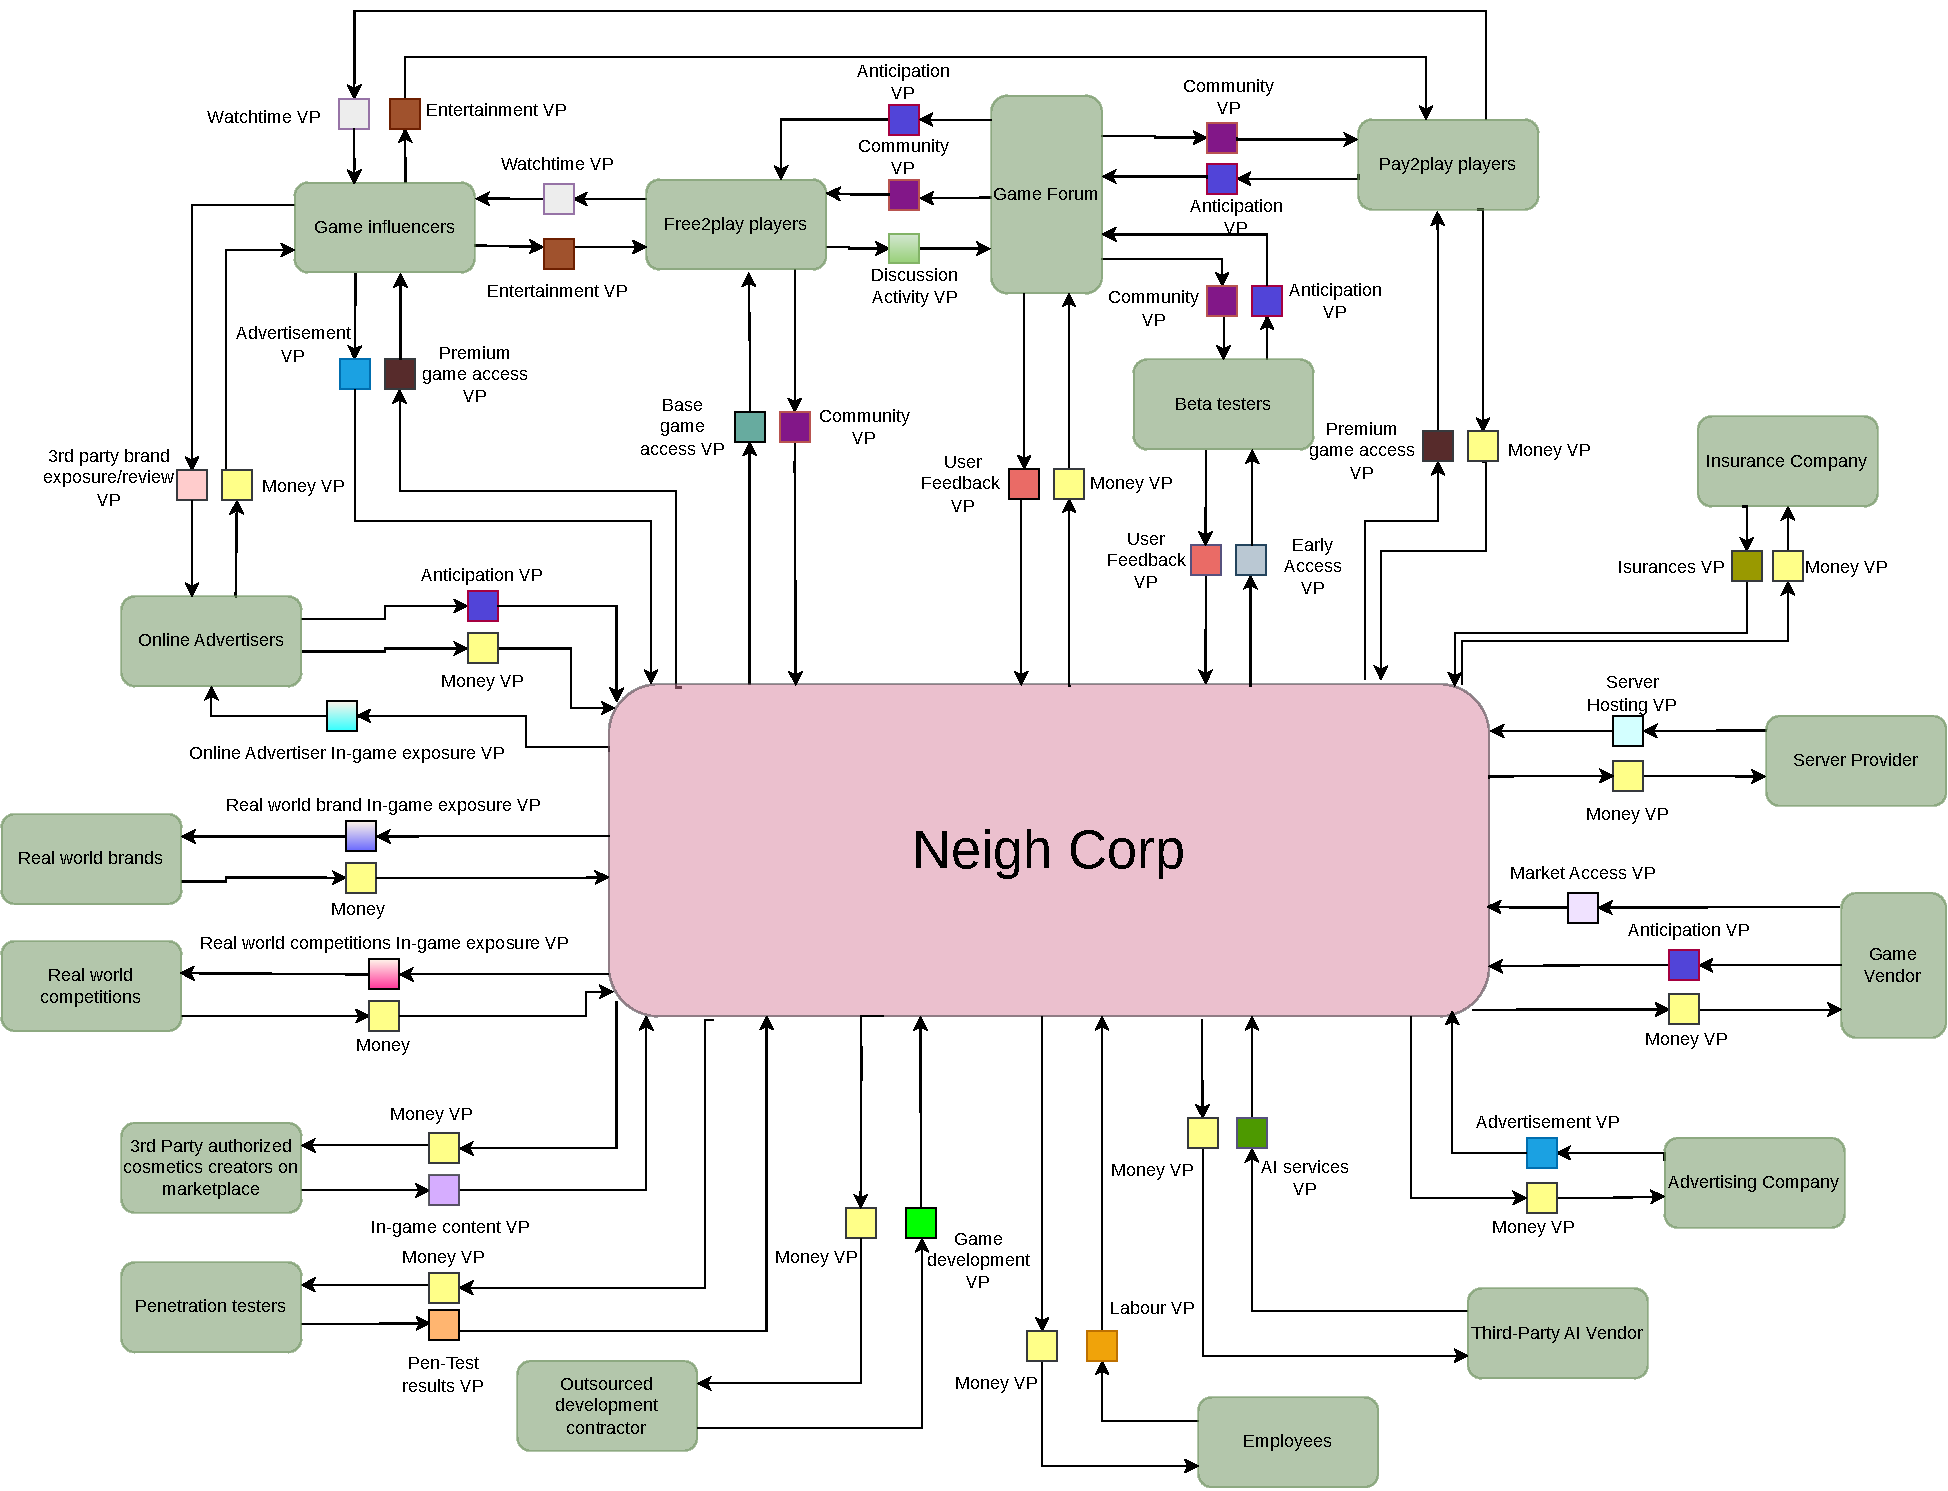
\includegraphics[width=1.6\linewidth]{figures/IS1_Project_VDML-Diagram.pdf}
    \caption{VDML Diagram of \textit{Neigh Corp}}
    \label{fig:VDML_diagram}
\end{figure}

\subsection{VDML Diagram}
\begin{figure}[H]
    \hspace*{-4cm}
    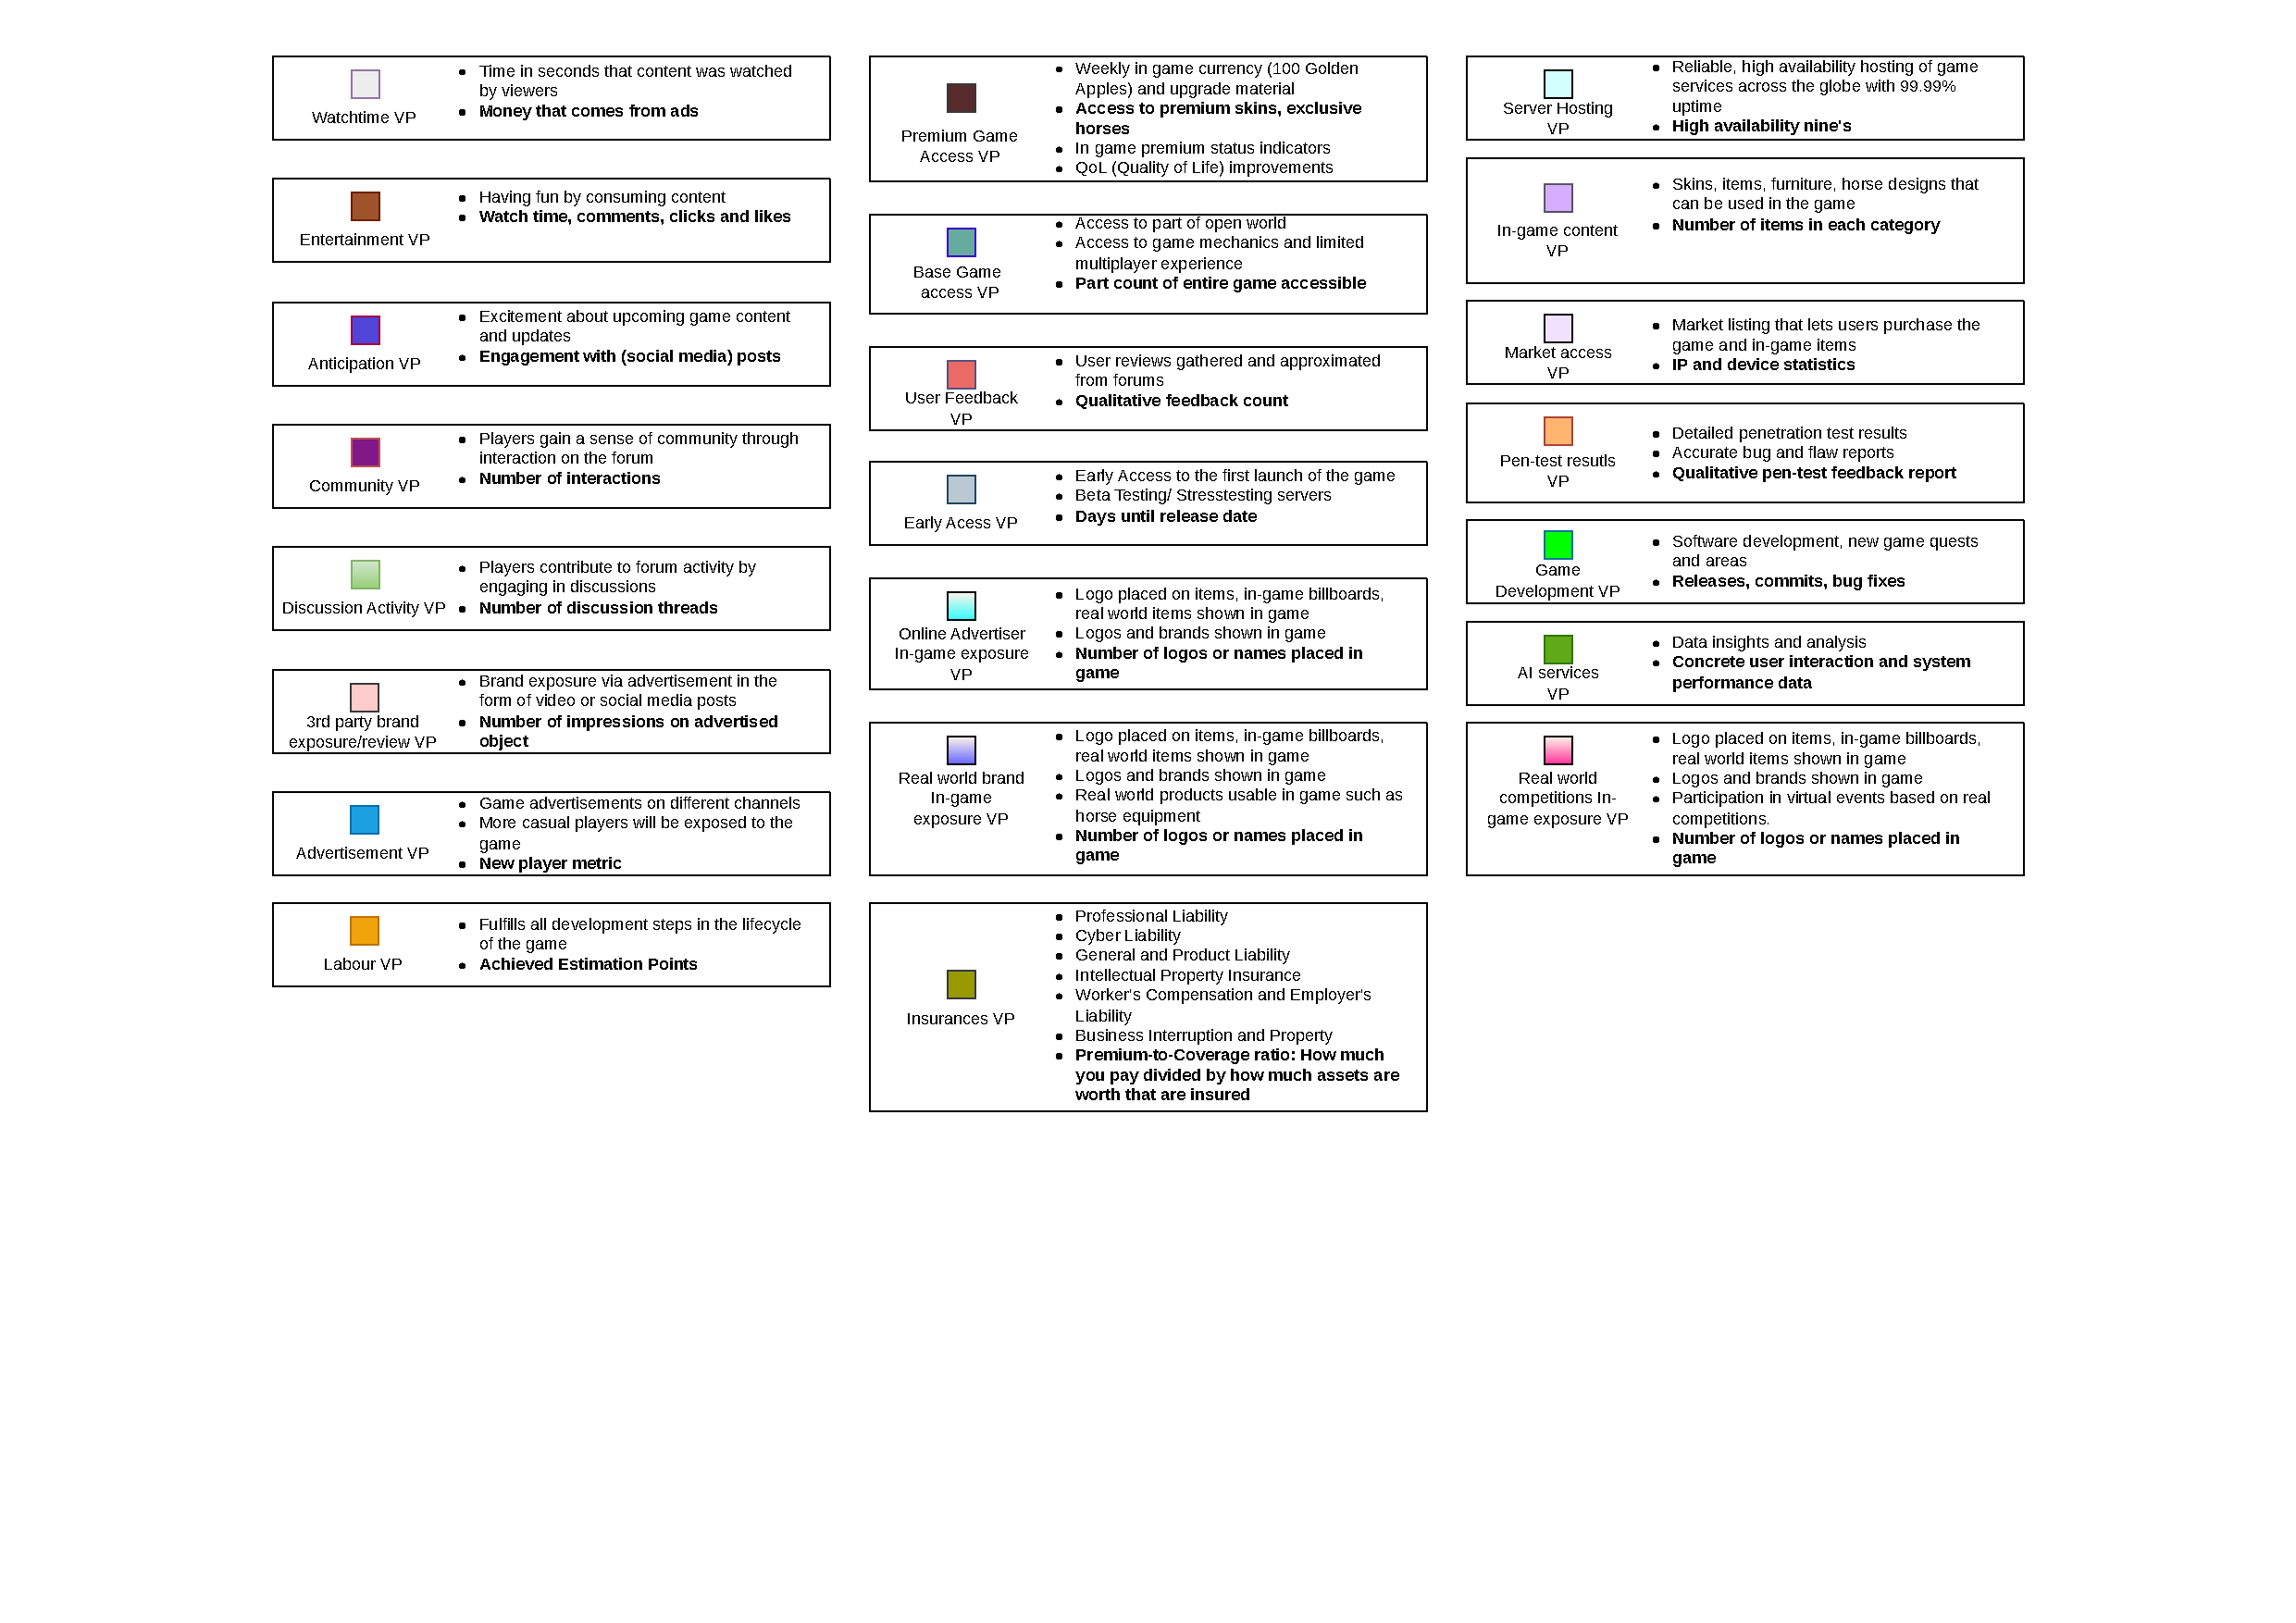
\includegraphics[width=1.6\linewidth]{figures/IS1_Project_VDML-Descriptions.pdf}
    \caption{VDML Descriptions of \textit{Neigh Corp}}
    \label{fig:VDML_description}
\end{figure}



\subsection{VDML Diagram Explained}
Seen above is the VDML diagram designed for Golden Meadows, featuring Neigh Corp as the central agent involved in the majority of value exchange processes. The diagram provides a comprehensive overview of the majority of actors involved in value propositions directly affecting the game.

The inclusion of individual agents was decided based on the previously-designed goal model as well as the actors typically engaged in the game development as well as MMO game maintenance processes. Each of the identified agents' involvements in a value proposition is briefly described below, as well as the agent itself where its name is not self-explanatory.

\subsubsection{Value Propositions between External Agents}

Several actors included on the VDML diagram are engaged in value exchanges without Neigh Corp's direct involvement, namely:

\begin{enumerate}
  \item \textbf{Free-to-play players as well as pay-to-play players and game forum}
  
    The \textit{Free-to-Play Players} actor, representing users of \textit{Golden Meadows} who do not conduct any in-game purchases, is engaged in a value exchange with \textit{Game Forum}, representing the online community where players can participate in conversations via forum posts. \textit{Pay-to-Play Players}, who are denoted as users actively purchasing in-game items and premium benefits, are, too, engaged in an identical value exchange with the exact same VPs. The following value propositions are involved in this relationship:
  
    \begin{enumerate}
    \item Community VP and Anticipation VP - given to the \textit{Players};
    \item Discussion Activity VP - given to the \textit{Game Forum}.
    \end{enumerate}

  \item \textbf{Game influencers and Free-to-Play as well as Pay-to-Play Players}

    The \textit{Free-to-Play} and \textit{Pay-to-Play Player} actors are also engaged in another value exchange with the \textit{Game Influencers} - an actor representing agents such as popular players, You-Tubers, as well as streamers contributing to the game's popularity. The value propositions are:

    \begin{enumerate}
    \item \textit{Watch Time VP} - given to the \textit{Influencers};
    \item \textit{Entertainment VP} - given to the \textit{Players}.
    \end{enumerate}

  \item \textbf{Game Influencers and Online Advertisers}

    The value exchange between \textbf{Game Influencers} and \textbf{Online Advertisers} involves the following value propositions:

    \begin{enumerate}
    \item Money VP - given to \textit{Game Influencers};
    \item Third-party Brand Exposure/Review VP - given to the \textit{Online Advertisers}.
    \end{enumerate}
\end{enumerate}


\subsubsection{Value Propositions involving Neigh Corp}

The majority of value exchange relationships depicted on the VDML diagram include Neigh Corp, described below:

\begin{enumerate}
    \item \textbf{Pay-to-play players}

    The exchange between pay-to-play players and Neigh Corp involves \textit{Money VP}, given to Neigh Corp, as well as \textit{Premium Game Access VP}, given to the pay-to-play players.

   \item \textbf{Game Forum}

   The \textit{Game Forum} agent receives the \textit{Money VP} from Neigh Corp in exchange for \textit{User Feedback VP}.

    \item \textbf{Free-to-play players}

    Neigh Corp receives \textit{Feedback VP} from the Players agent, defined on the diagram seen above, in exchange for \textit{Base Game Access VP}.

    \item \textbf{Beta testers}

    \textit{Beta Testers} receive \textit{Early Access VP}, and in turn, Neigh Corp receives \textit{User Feedback VP}. Both value propositions are given concrete definitions on the image seen above, below the VDML diagram.

    \item \textbf{Game Influencers}

    \textit{Game Influencers} receive \textit{Premium Game Access VP} in exchange for \textit{Advertisement VP}.

    \item \textbf{Online Advertisers}

    \textit{Online Advertisers} are engaged in a value exchange with Neigh Corp, receiving the \textit{Online Advertiser In-game exposure VP}. The actor, in turn, gives \textit{Money VP} as well as \textit{Anticipation VP}.

    \item \textbf{Real-world brands}

    \textit{Real-world brands} provide Neigh Corp with the \textit{Money VP}. The actor receives \textit{Real world competitions In-game exposure VP} (see definition).

    The \textit{Real-world brands} actor represents real-life companies wishing to engage in a partnership with Neigh Corp, provided with ad placement within the game in exchange for a monthly or one-time fee, decided on a case-by-case basis and the duration of ad placement.

    \item \textbf{Third-party authorized cosmetics creators on marketplace}

    The actor represents individual users or groups of people engaged in the development of in-game cosmetics. In exchange for the provided \textit{In-Game Content VP}, the actor receives \textit{Money VP} from Neigh Corp.

    \item \textbf{Penetration testers}

    Penetration testers receive \textit{Money VP} from Neigh Corp in exchange for conducting penetration tests in order to identify potential security vulnerabilities within the company's infrastructure, represented by the \textit{Pen-Test Results VP}.

    \item  \textbf{Outsourced Development Contractor}

    Third-party developers hired by Neigh Corp for various development tasks are represented by this agent, receiving the \textit{Money VP} in exchange for \textit{Game Development VP}.

    \item \textbf{Third-Party AI Vendor}

    \textbf{Third-Party AI Vendors} is an agent representing companies providing Neigh Corp with a miscellaneous set of AI tools, for instance, copilots, agents, or data gathering software. The provided \textit{AI Services VP} is exchanged for \textit{Money VP}.

    \item \textbf{Advertising Company}

    The advertising company actor receives \textit{Money VP} from Neigh Corp in exchange for the advertising services the agent provides, represented by the \textit{Advertisement VP}.

    \item \textbf{Game Vendor}

    The \textit{Game Vendor} agent, denoting a game marketplace providing companies with a platform to sell their product on, exchanges \textit{Anticipation VP} for \textit{Money VP}, anticipation in this context meaning teasers being released ahead of the game's or its update's release.

    \item \textbf{Server Provider}

    The \textit{Server Provider} agent gives Neigh Corp the \textit{Server Hosting VP}, in turn receiving \textit{Money VP}.

    \item \textbf{Insurance Company}

    \textit{Insurance Company} provides Neigh Corp with the \textit{Insurances VP}, which represents one or more active insurance agreements. Neigh Corp pays for said insurance with the \textit{Money VP}.

    \item \textbf{Employees}

    The agent representing \textit{Employees} receives \textit{Money VP} from the company in exchange for \textit{Labour VP}.

    \item \textbf{Payment Provider}

    The agent representing \textit{Payment Providers} receives \textit{Money VP} from the company in exchange for \textit{Payment Service VP}.
    

\end{enumerate}






\section{Goal Design}
This section is to show the goals of the company. The goals shall be clearly related to the value network analysis in Section 1. In order to identify relevant goals, the project group shall make use of the five forces model and generic strategies of Michael Porter (see links on the page “Reading Resources” at the course web site). It is recommended that Strategy maps be used to structure the goal model (see link on the same page).

\subsection{Goal Model}

\begin{figure}[H]
    \hspace*{-4cm}
    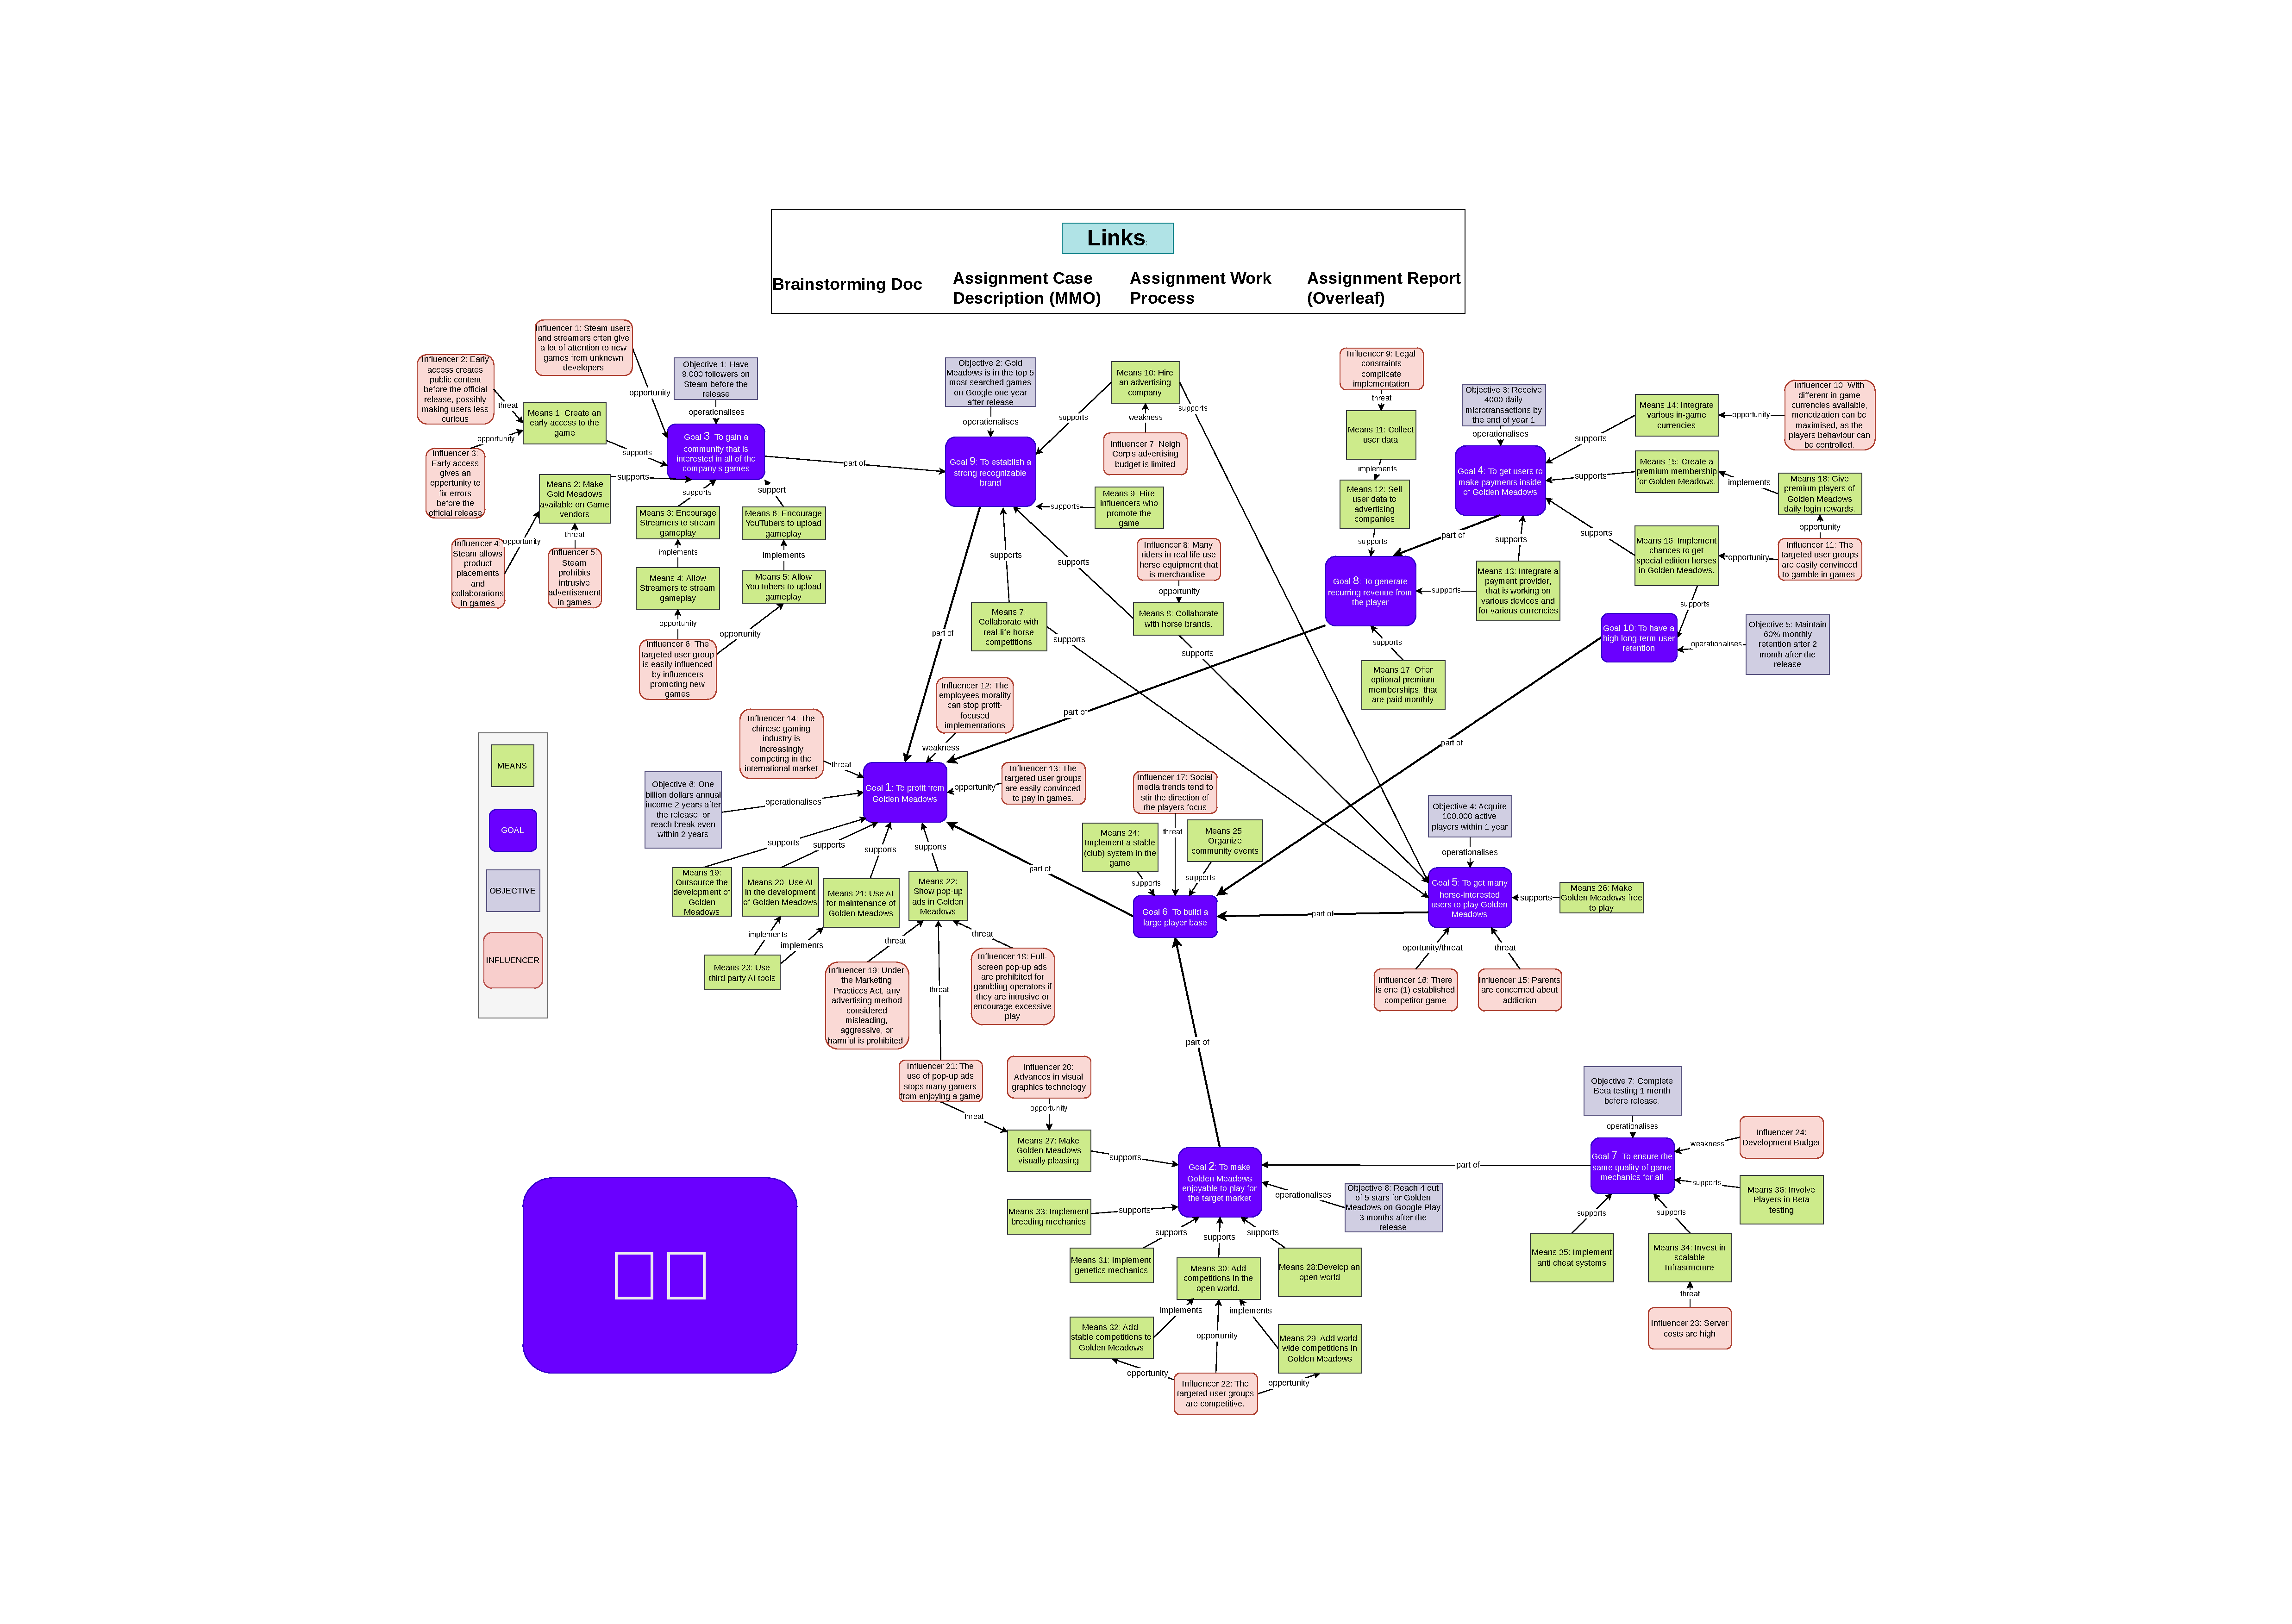
\includegraphics[width=1.6\linewidth]{figures/IS1_Project_Goal_model-Page-1.pdf}
    \caption{Goal model for \textit{Neigh Corp}}
    \label{fig:Goal_model}
\end{figure}

\subsection{Goal Model Explained}
% Include a textual description of the BMM model that explains it and shows how it is related to the components of the five forces model.

\autoref{fig:Goal_model} shows the goal model for Neigh-corp. It describes the overarching goals, subgoals, influencers that affect these goals and the means that can help achieve them. The coloured border around the boxes in the diagram indicate which dimension of value creation in the company these belong to, in accordance with \cite{kaplan2004strategy}. Which colour corresponds to which level is shown in the diagram next to the legend. The levels shown in the diagram are ordered in accordance with the levels in the generic strategies, ranging from financial goals at the top to concrete technologies at the bottom. Influencers are modelled outside any perspective, as these can impact across several categories and are not influenced by the company.

The first level, named "Learning \& Growth" contains the technologies used in the company. This level supports the one above it, "Internal Business Processes" which lists the methods and processes the company uses to create value. The "Customer" perspective contains the most elements and describes how these processes create value for the customer, and the final "Financial" level shows how all these elements combine to fulfil the most important monetary goals in the company such as profit and recurring revenue.

The goal model was created with the previously shown \autoref{fig:VDML_diagram} diagram in mind and in accordance with Porters five forces \cite{quickmba_porter} and Porters generic strategies. %\cite{wikipedia_porter_generic_strategies}.
Each of porters five forces are listed below with an analysis of which parts of the diagram belong to it, which Generic strategy is used to combat its force and the reasoning behind their Strategy maps classification.  The overarching approach for Golden Meadows is differentiation, as the target customer group for this game is rather niche.\\

\textbf{Competitive rivalry:}
This force measures how many competing products there are on the market. A large number of competitors results in a greater force. Influencers 14 and 16 measure this force. They indicate that there is increasing competition from Chinese gaming companies and that there is one established competitor with high market share and high cost of switching. This makes the competitive rivalry force comparatively strong, since the potential for new competitors emerging has increased, and potential customers experience a high cost of switching to Golden Meadows. 

A number of goals and means are in place to combat this force. Means 26 is about making Golden Meadows free to play, as shown in the VDML \autoref{fig:VDML_diagram}. This makes the game accessible to new users at no cost and therefore lowers upfront switching cost to zero.

Goal 9, establishing a strongly recognizable brand also combats this through establishing Golden Meadows individual identity. While competitors can copy graphics, the means that go into this goal, such as collaborating with real-life horse related brands and hiring influencers, are harder to replicate. These means and goals relate to the VDML Game influencers and actor that provide Neigh Corp with excitement for game content and updates.

% inf 16 and inf 14, goal 9 and 2 more

\textbf{Bargaining Power of Buyers:}
This force measures how much power the buyers have. The influencers in the goal model that show weakness in this force are influencer 11 and 14, which state that the target group is easily convinced to pay and gamble. The factors that strengthen this force are influencer 15 and 21, which state that parents control purchases of younger players and that pop-up ads can decrease their game enjoyment.

inf 11, 13, 15, 21

\textbf{Bargaining Power of Suppliers}
inf 4,5, 23, 25, 26

\textbf{Threat of New Entrants}
inf 1, 20 (threat to goal 2 because it can raise graphical fidelity expectations), 27 (easier market entry for competitors)

\textbf{Threat of Substitutes}
inf 28, 29, 30 (but there it is good for us since it weakens the porter force)

\textbf{Generic strategies}
How do we combat these five forces?
OBS: One consistent way of combating all five. Need to defend against each.
Our main approach: Niche

Market approach is grassroots/influencer based






\section{Process Design}
This section is to show the processes of the company. The processes shall be clearly related to the value network analysis in Section 2 and the goal design in Section 3.

\subsection{Exchange and Conversion Processes in REA}
\subsubsection{Conversion Processes}
\begin{center}
\begin{landscape}
    \begin{figure}[H]
    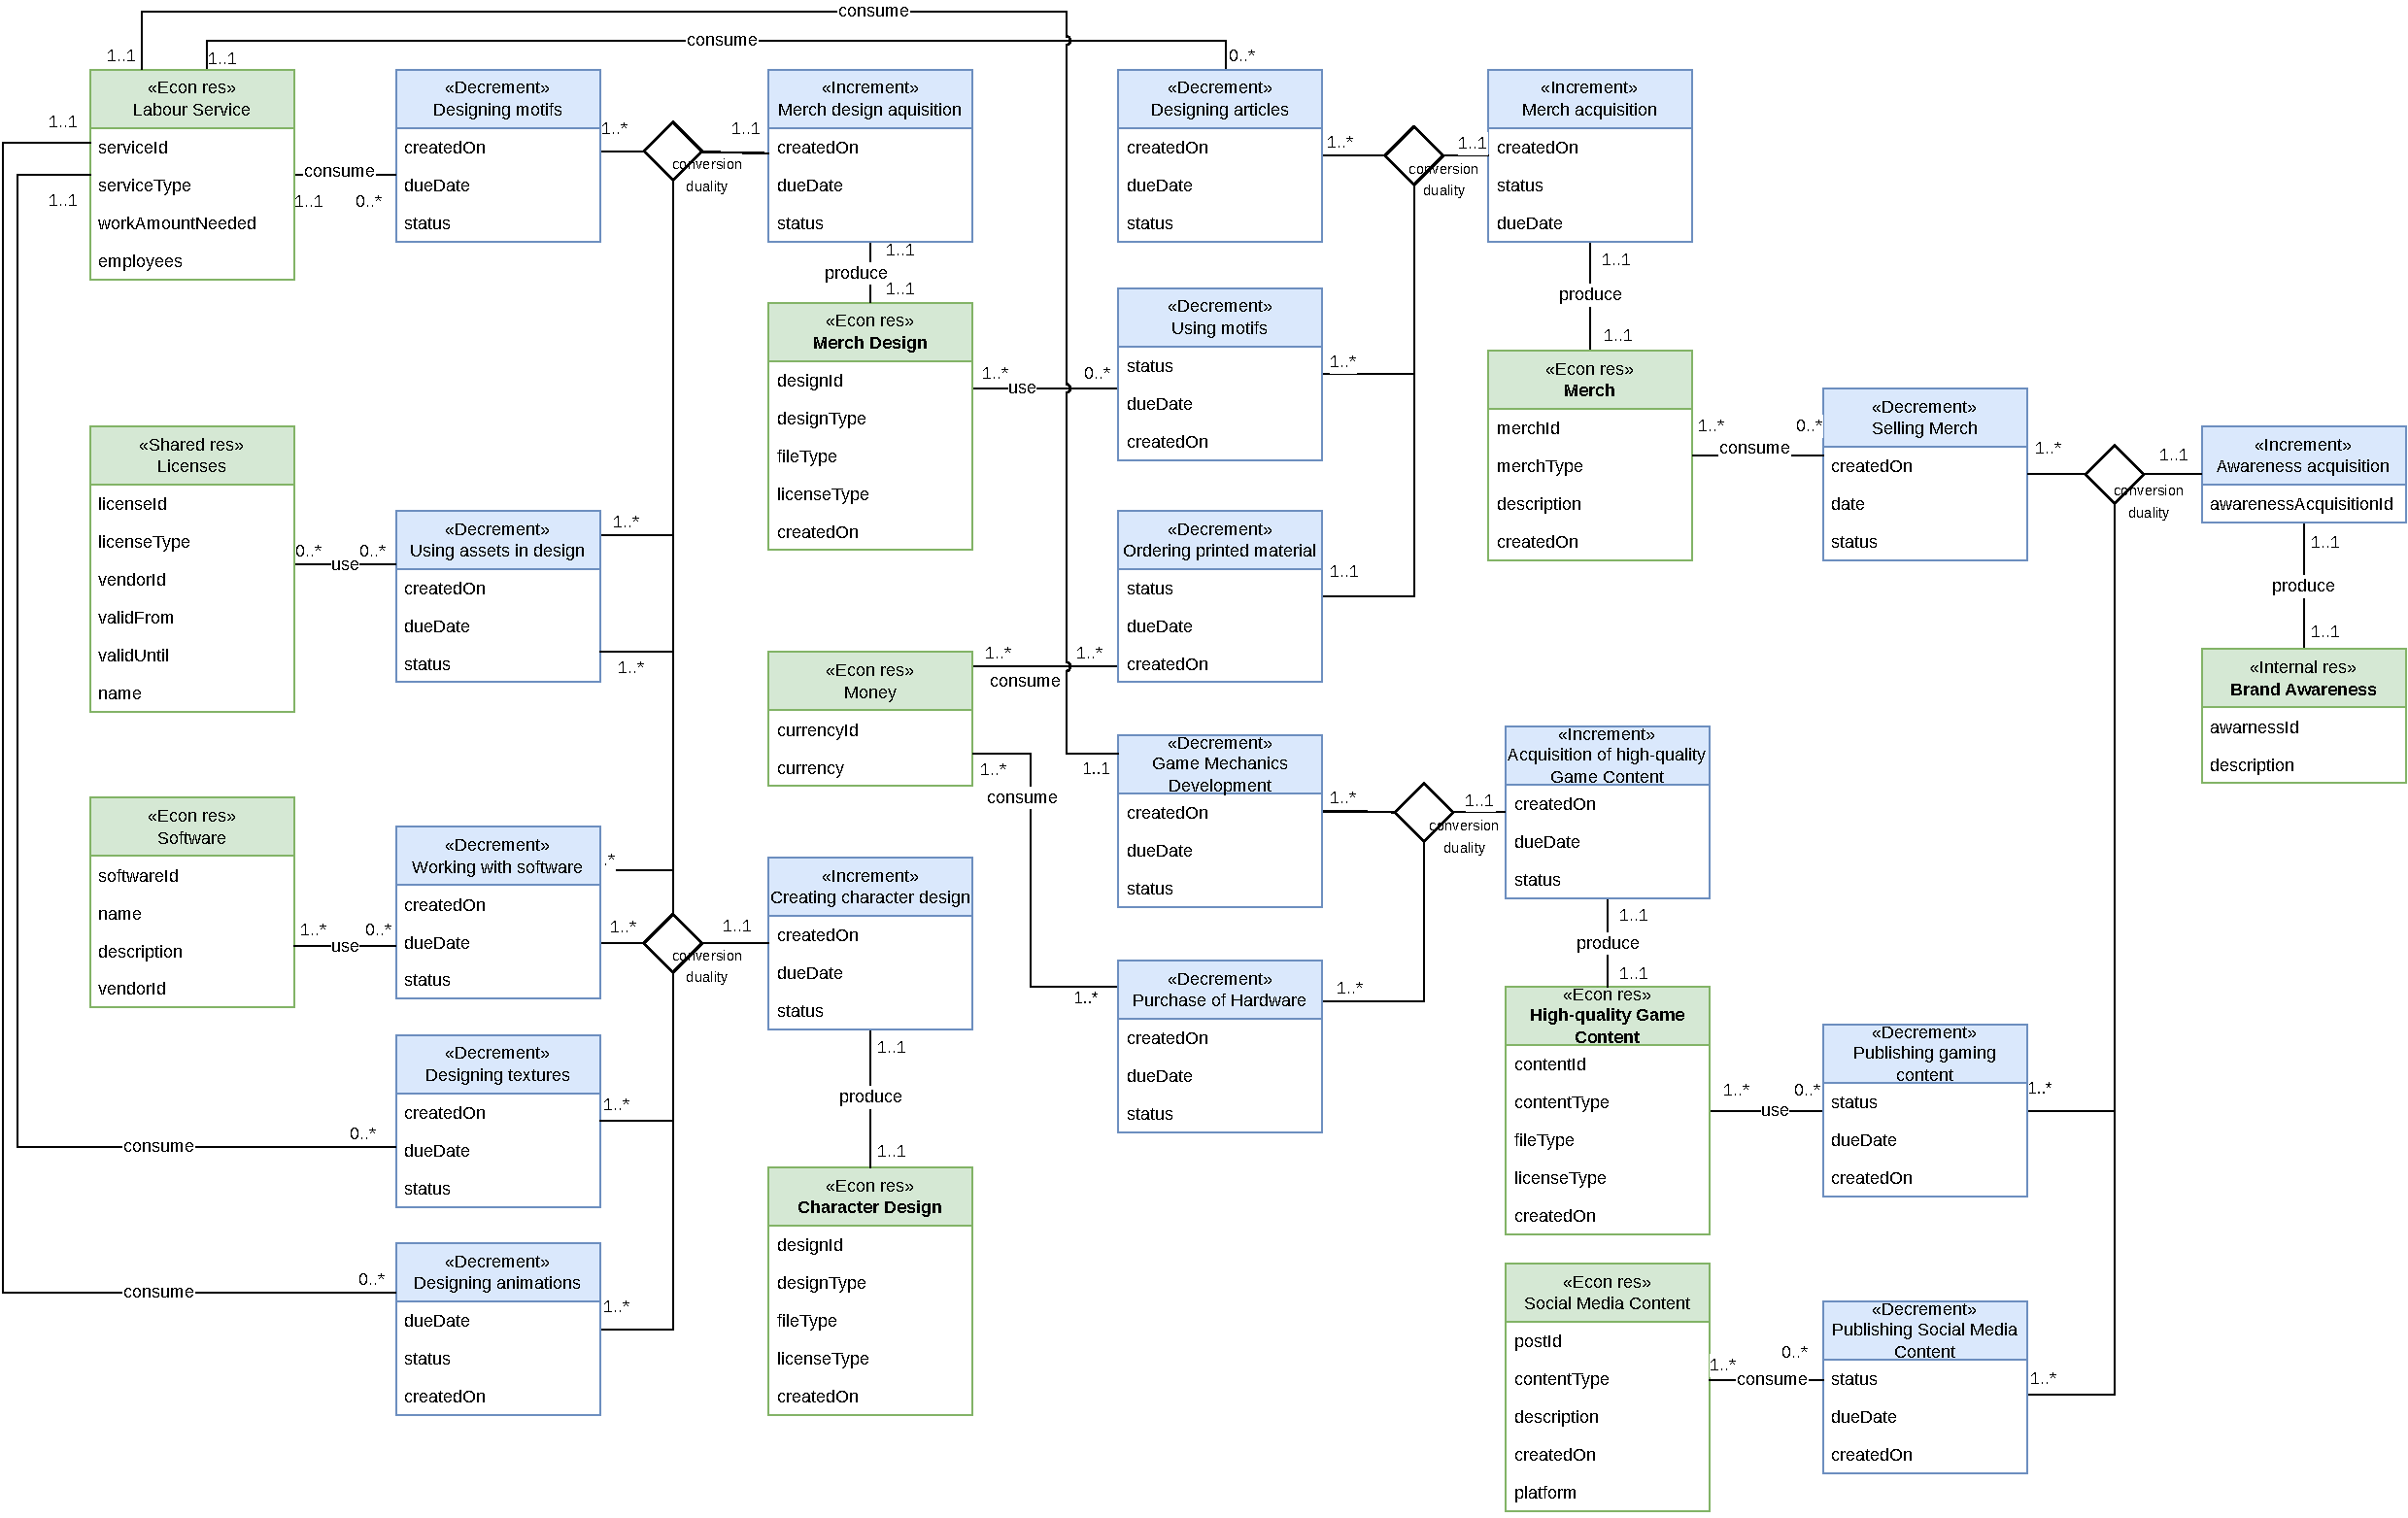
\includegraphics[width=1.3\linewidth]{figures/IS1_Project_REA-Conversion.pdf}
        \caption{Conversion processes \textit{Neigh Corp}}
        \label{fig:Conversion_process}
    \end{figure}
\end{landscape}
\end{center}

Seen above is the diagram depicting every conversion process Neigh Corp is involved in. The conversion processes included are as follows:

\begin{enumerate}
    \item \textbf{Merch Design Conversion Process}
    
    
        The economic event \textit{Designing motifs} decrements the \textit{Labour Service} resource with a 1..1 to 0..* multiplicity, meaning that one and only one labour service, representing the act of employees working, can simultaneously be engaged in many motif designs, or as few as zero. The resource is \textbf{consumed}.
        
        \textit{Working with Software} decrements \text{software} in a \textbf{use} relationship, i.e., the software is not permanently destroyed in the process and can be used again in future processes. The software may be used by zero or many of these events, and the event itself may be using one or many software resources, as the event name itself implies at least one software resource has to be used.
    
        Lastly, the event \textit{Using assets in design} decrements \textit{Licenses} - the resource representing licenses that may be necessary to acquire in order to use certain design elements (assets, as the event name implies). Zero or many licenses may be necessary as there is no guarantee copyrighted material will be used. For that reason, licenses are also engaged in zero-to-many of these events, as they may or may not be used by many asset design use events.
    
        Finally, each event is engaged in a one-to-many relationship with the conversion process, as each of the events may need to occur multiple times to finalise a merchandise design. The events are converted into the \textit{Merch Design Acquisition} increment event, which produces the final \textbf{Merch Design} resource.

    \item \textbf{Character Design Conversion Process}


        The same two resources described in the previous process are engaged in this conversion process as well, using identical multiplicities, with the exception of \textit{software}.
    
        \textit{Labour Service} is consumed in a 1..1 to 0..* relationship with both the \textit{Designing Textures} and \textit{Designing Animations} decrement events. The labour service, i.e. the employees, may not necessarily be engaged in either of these events, hence the multiplicity of 0..*, but if these events are taking place, labour service must always be consumed by both of them. The \textit{Working with software} decrement event takes place once again, engaged in the same \textbf{use} relationship with \textit{software} as before. The three decrement events are converted into the \textit{Creating Character Design} increment event, which produces \textbf{Character Design}.

    \item \textbf{Merch Conversion Process}

        The corresponding decrement events of the process are as follows:

        \textit{Designing Articles} - the event consumes \textit{Labour Service} in a 1..1 to 0..* relationship, the multiplicity reasoning being identical to what was discussed in the previous conversion processes regarding said resource. 
        
        The \textit{Merch Design} resource produced by the first conversion process is used by the \textit{Using motifs} economic event in a 1..* to 0..* relationship, meaning that one or many merchandise designs may be used by many of these events at once, but they don't have to be, either because there is no event taking place or because the merchandise design simply remains unused. If, however, the event is happening, at least one motif has to be used. 

        Lastly, \textit{Money} economic resource is consumed by the \textit{Ordering printed material} event in a 1..1 to 1..1 relationship.

        Finally, the three economic events are converted into the \textit{Merch Acquisition} event which produces the \textbf{Merch} resource.

    
    \item \textbf{High-quality Game Content Conversion Process}

        Two economic decrement events are engaged in this conversion process, the first one being \textit{Game Mechanics Development}, which consumes the \textit{Labour Service} resources in a 1..1 to 0..* relationship, meaning that the employees represented by the resource are not always working on a new game mechanic, and if they are, they might not be working on only one. 
        
        The second event is \textit{Purchase of Hardware}, which consumes \textit{Money} in a 1..1 to 1..1 relationship (i.e., one purchase requires one sum of money representing the sum necessary for one purchase, and you cannot pay for more than one purchase using a sum representing one purchase payment).

        The two events are converted into the \textit{Acquisition of High-Quality Game Content} event, which produces the \textbf{High-Quality Game Content} resource.

    \item \textbf{High-quality Game Content Conversion Process}

    Three economic events participate in this conversion process. The first decrement event, \textit{Selling Merch}, consumes the \textit{Merch} resource produced in the earlier conversion process in a 1..* to 0..* relationship, meaning that if merchandise is being sold, at least one unit of merchandise must actually be consumed in the process, though not limited to one. Merchandise itself does not necessarily have to be in the process of being sold, and it can be sold by multiple \textit{Selling Merch} events given that more copies can be theoretically made.

    Moving on, the \textit{Publishing Game content} decrement \textbf{uses} the \textit{High-Quality Game Content} produced in the previous process, the multiplicities being 1..* to 0..*. This implies that at least one unit of high-quality game content must be used by the event, as its very name suggests, though there is no set limit. Meanwhile, \textit{High-Quality Game Content} can exist as a unit without having to be actively used, hence the 0..* on the right side.

    The last economic event is \textit{Publishing Social Media Content} which consumes the \textit{Social Media Content}, the reasoning being that once a social media post is made public, publishing it again will be redundant, as it will have already used up its value as a form of advertisement. The multiplicities between the resource and the event are 1..* to 0..*, using roughly the same logic as in the previous resource-event relationship (the event name implies at least one resource has to be used for the event to occur, and the resource can exist without being engaged in the event). 

    The three events are converted into the \textit{Awareness Acquisition} increment event, which, finally, produces \textbf{Brand Awareness}, representing how well-known Neigh Corp's company name is, as well as the game itself. 
        

    
    

    

    
\end{enumerate}

\subsubsection{Exchange Processes}
ADD 8 DIAGRAMS\\
We modelled the following Exchange Processes:

Neigh Corp - Server Hosting Provider (Server Hosting Service)
Neigh Corp - Pentesting Service Provider (Pentesting Service)
Neigh Corp - Outsourced Game Development Contractor (Game Development Service)
Neigh Corp - Player (Premium Pass)
Neigh Corp - Player (Base Game Access)
Neigh Corp - Employee (Labour Service)
Neigh Corp - Tax Agency (Money)
Neigh Corp - Insurance Company (Rights to claim insurance)

\subsection{Detailed Processes in EPC}
Include a number of detailed process models, expressed as EPC diagrams. The processes should include sales and procurement. The process models should show actions of individual actors and handle alternatives and exceptions. It is recommended to make each process diagram small by using the decomposition mechanisms of EPC diagrams.

\subsubsection{Sales Process}

\begin{center}
    \begin{figure}[H]
    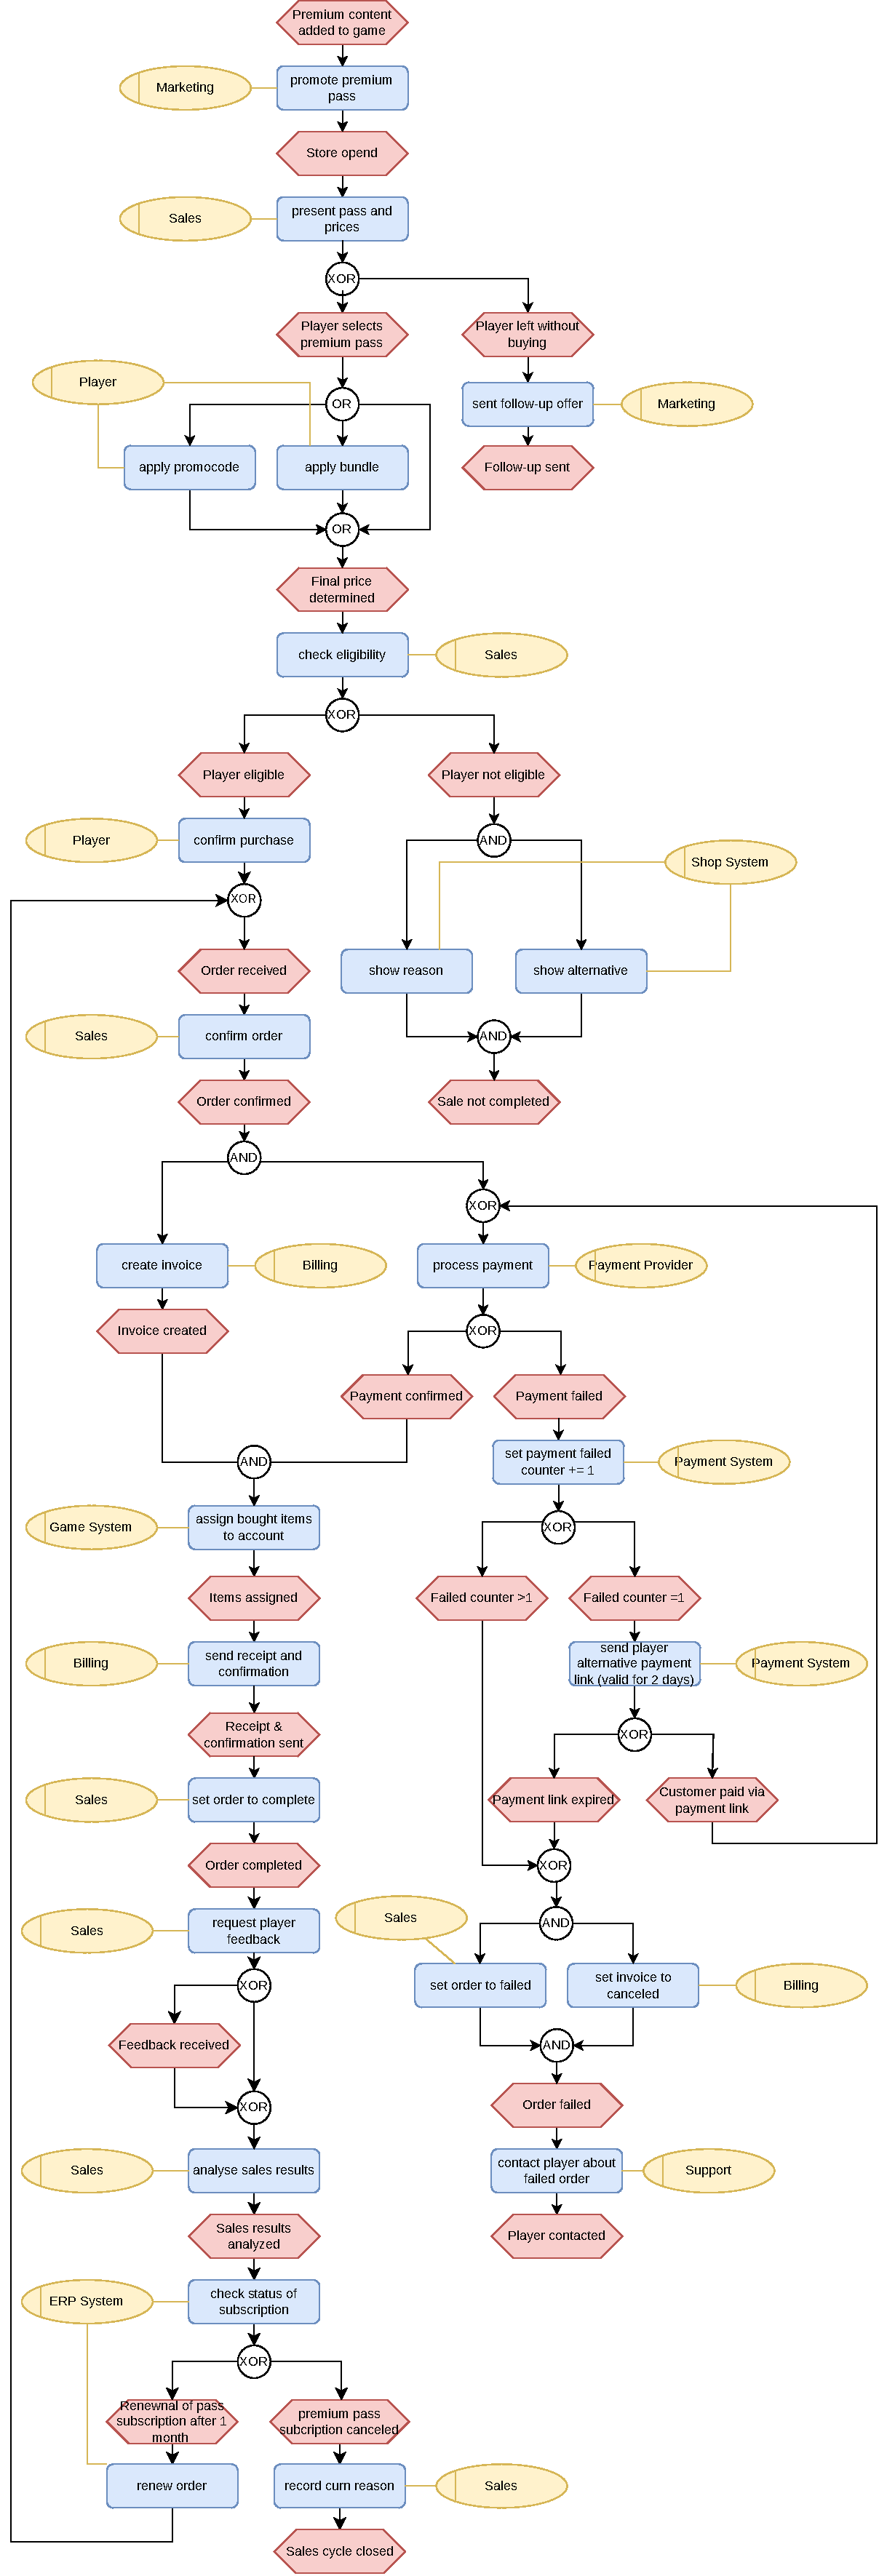
\includegraphics[width=\linewidth,
                     height=0.85\textheight,
                     keepaspectratio]{figures/IS1_Project_EPC_Model-Sales-Process.pdf}
        \caption{Conversion processes \textit{Neigh Corp}}
        \label{fig:Sales_process}
    \end{figure}
\end{center}

Involved in the Sales Process are the organisational units Marketing, Sales, Player, Billing, Payment Provider, Shop System, and the ERP System.

DESCRIPTION

\subsubsection{Procurement Process}
\begin{center}
    \begin{figure}[H]
    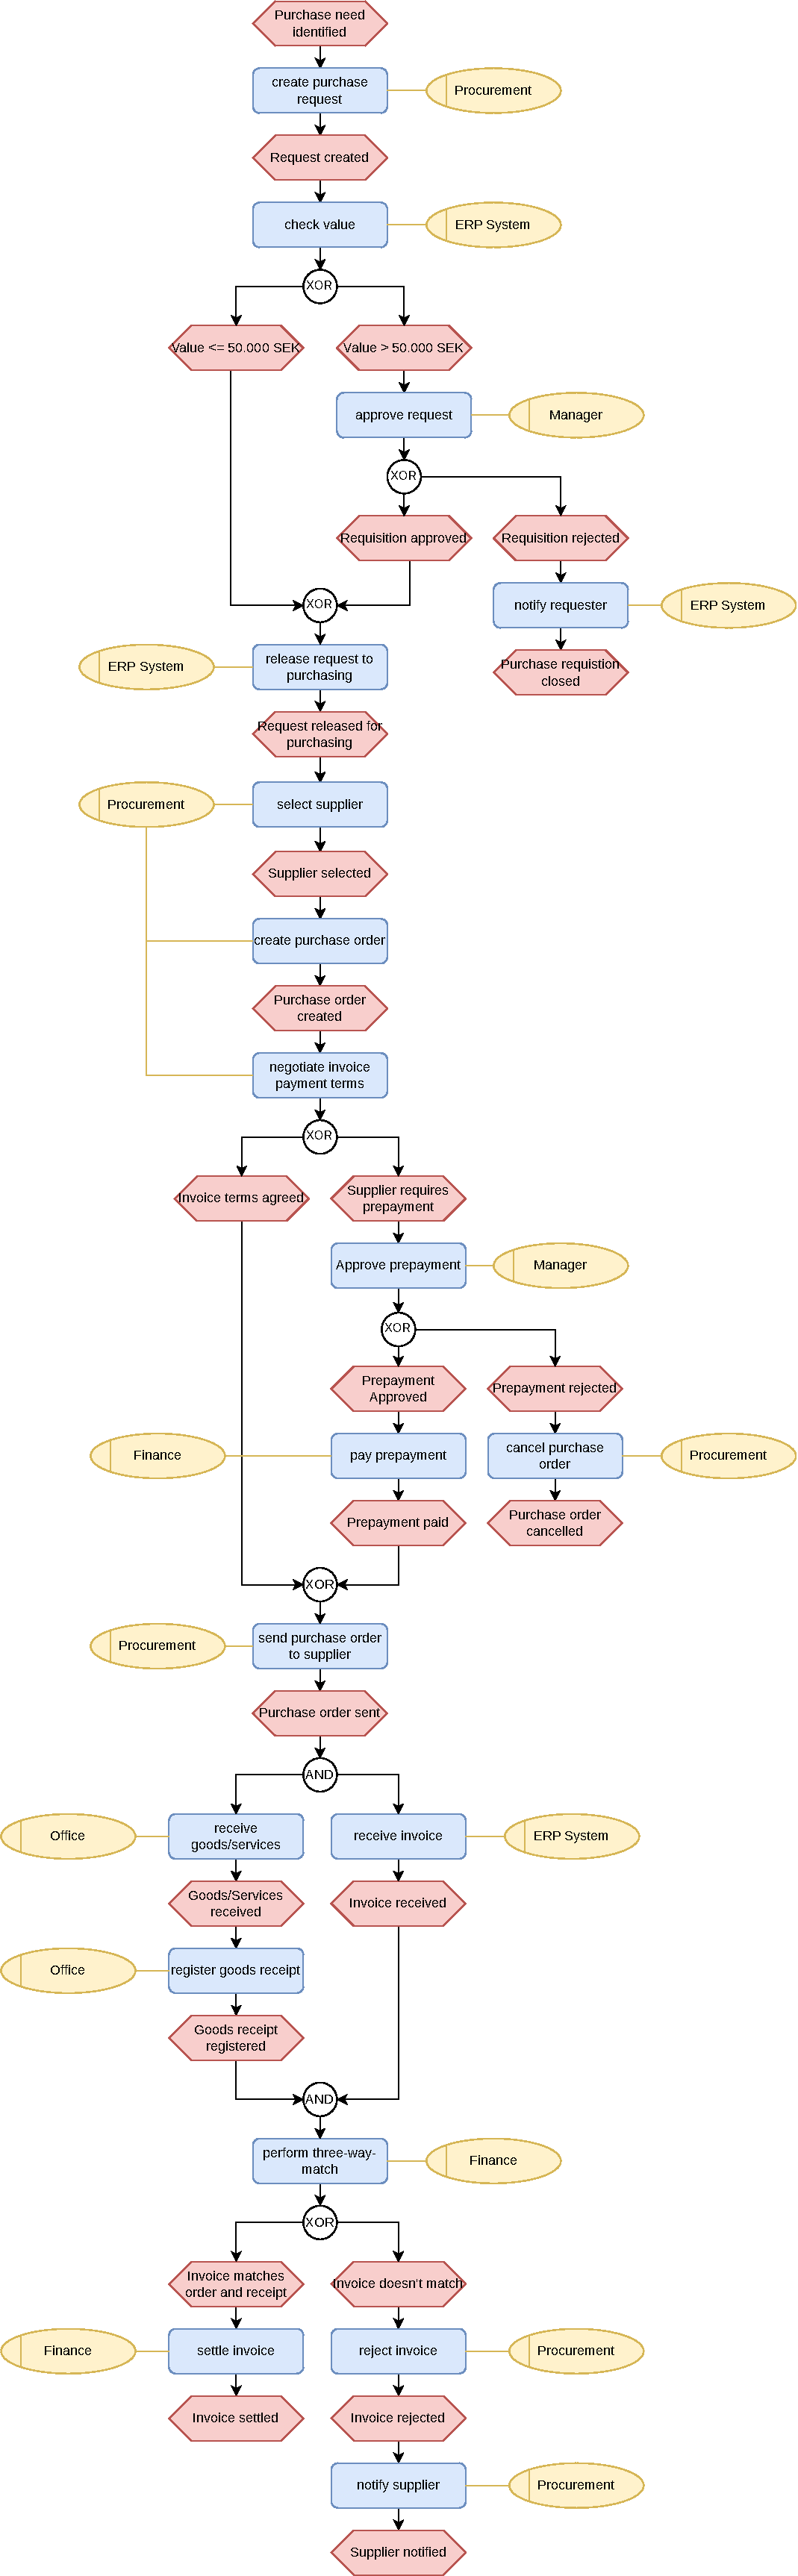
\includegraphics[width=\linewidth,
                     height=0.85\textheight,
                     keepaspectratio]{figures/IS1_Project_EPC_Model-Procurement-Process.pdf}
        \caption{Conversion processes \textit{Neigh Corp}}
        \label{fig:Sales_process}
    \end{figure}
\end{center}

In the Procurement Process, the organisational units Procurement, ERP System, Manager, Office, and Finance are involved.

The process starts when the company identifies a need to purchase goods or services. The Procurement department creates an internal purchase request, which is then registered. The ERP system checks the value of the request. If the value exceeds SEK 50,000, a manager reviews the request and either approves or rejects it. Requests of SEK 50,000 or less continue without managerial approval.
Approved requests and requests that do not require approval are released for purchasing. The Procurement department then selects a supplier. If the manager rejects the request, the ERP system notifies the requester and the case is closed.

After the supplier is selected, the Procurement department creates a purchase order and negotiates the payment terms with the supplier. If the terms are agreed without prepayment, the order is sent to the supplier. If the supplier requires prepayment, a manager must approve it. If approved, the Finance department pays the prepayment, and Procurement then sends the purchase order to the supplier. If the manager rejects the prepayment, Procurement cancels the purchase order and the process ends.

After the purchase order is sent, the Office receives the goods or services and registers the goods receipt. In parallel, the ERP system receives the invoice. Both steps must be completed before the process continues. The Finance department then compares the purchase order, the goods receipt and the invoice through a three-way match. If they match, Finance settles the invoice. If they do not match, the Procurement department rejects the invoice and notifies the supplier.

\subsubsection{Hiring Process}
\begin{center}
    \begin{figure}[H]
    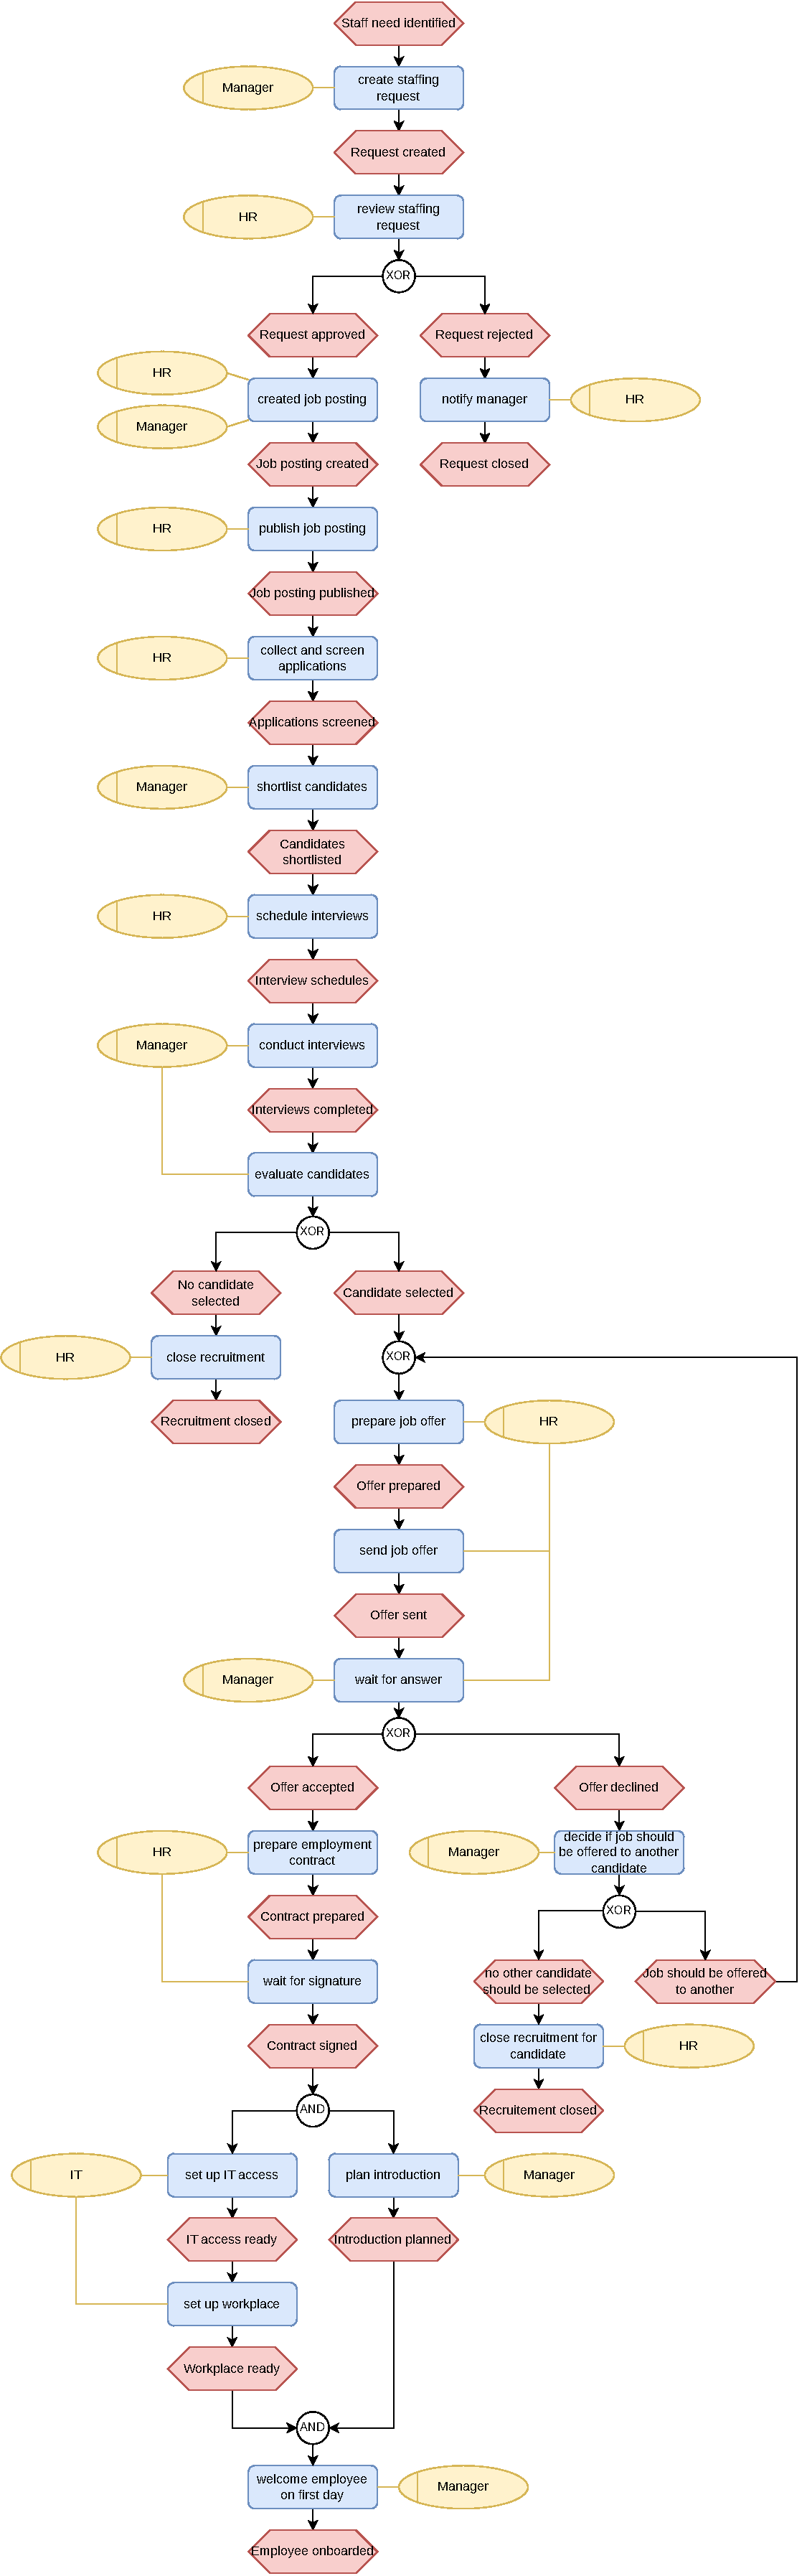
\includegraphics[width=\linewidth,
                     height=0.85\textheight,
                     keepaspectratio]{figures/IS1_Project_EPC_Model-Hiring-Process.pdf}
        \caption{Conversion processes \textit{Neigh Corp}}
        \label{fig:Sales_process}
    \end{figure}
\end{center}


In the Hiring Process, the involved organisational units are HR, Manager, and IT.

When a need for staff is identified, the Hiring Process begins. A manager creates a staffing request which is being reviewed by HR. If they do not approve, the manager is notified and the request will be closed. If they approve, they create a job posting with the manager that they publish. Then, the applications will be collected and screened by HR. The manager shortlists the candidates and HR schedules interviews. The manager conducts interviews and evaluates the candidates. If there are no fitting candidates to select, HR closes the recruitment. If one candidate get selected, HR prepares a job offer, sends it to the candidate and HR and the manager wait for an answer. If the candidate declines the offer, the manager decides whether to close the recruitment if no other candidate should be selected, or if the job should be offered and sent out to another candidate.
When an offer is accepted by a candidate, HR prepares and sends out an employment contract. After the contract is signed, IT sets up IT access and sets up the workspace while the manager plans an introduction for the new employee.
Then, the new employee is welcomed on their first day by the manager. The process is completed now that the employee is onboarded.


\subsection{Relationships between Models}
Include one or several tables that visualize the relationships between the models introduced in this section and the models in the previous sections. The tables should help to answer the following questions: 
\begin{itemize}
\item How does the design of the processes help in fulfilling the goals of the company? 
\item What are the relationships between the exchange and conversion processes and the EPC models? 
\item What are the relationships between the EPC models and the VDML diagram?
\end{itemize}

\section{IT Architecture Design}
This section is to show the IT architecture of the company. The IT systems to be used in the company are to be specified, including BPMS, CRM, ERP, DW, BI tools, dashboard, and
KM. The use of EAI and decision support systems (BI, DW and Dashboards) shall also be discussed. The IT architecture shall be documented graphically in a diagram showing the systems
and the data flows between them, representing systems as nodes and data flows as labelled arrows. The relationships between the systems and the business processes they support shall be made explicit.

\section{Business Performance Management}
This section is to introduce the key performance indicators (KPI) for measuring and analysing the business processes of the company. 

\subsection{Leading and Lagging KPIs}
Include between five and ten leading and lagging indicators. Each indicator shall be described in an indicator template consisting of at least the following parts: name of the indicator, definition of the indicator, which goal(s) in the company’s goal model that the indicator is related to, target values, which part of a business process (i.e. which activity) the indicator measures, which IT system that will be the data source for the indicator, and which type of IT solution will feed the dashboard system with data from the source system. Ensure that the descriptions are consistent with the IT architecture in Section 5.

\subsection{Evaluation of KPIs}
Include an evaluation of the KPIs from the previous subsection, based on the article by Eckerson. 

\section{Enterprise Architecture Evaluation}
In other parts of the work, you have designed the organization from several perspectives: goals, processes, IT architecture, and so on. All of these combined converge towards an Enterprise Architecture (EA). A key component of EA is capability, an ability and capacity that enable an enterprise to achieve a business goal in a certain context. In this light, your task is to design one capability based on the models already created. The first step is to fill in the capability elicitation template in terms of relevant goals, KPIs, context, business process variants. This should be followed by a graphical design of a capability model, for instance, by introducing links between the newly developed capability and the corresponding constructs in other models.



\printbibliography
   




\end{document}
